\chapter{Evaluation}\label{chap:evaluation}
FlyTrap imposes an overhead to vanilla MQTT brokers. It is vital to ensure that the added layer of authentication does not severely impact the operation of the broker, as MQTT is a time-sensitive protocol, requiring frequent and rapid responses. In this chapter, we present experiments to measure latency caused by FlyTrap, the operational cost on a public blockchain and also reflect back to user stories to ensure that FlyTrap fulfils the specified needs. In the end, we reflect on the findings and answer the stated research questions, determining the feasibility of the solution in the real world.

\section{Experimental Design}
This section includes details on how the experiments were designed and what the main motivations behind each of them were, along with a description of the hardware and the software used, to ensure reproducibility.
\subsection{Research Question(s)}
Four separate aspects of the implementation were investigated and these can be summarised with the following research questions, which each of the subsequent section attempts to answer:
\begin{enumerate}
  \item How significant is the performance hit by proxying the connection through FlyTrap, as opposed to directly connecting to the broker (further referred to as state-of-the-art)?
  \item How does FlyTrap scale as the number of concurrent requests goes up?
  \item How expensive would the operation of FlyTrap be on a Proof-of-Work type of blockchain network?
  \item How does FlyTrap address the problems highlighted by the use-case scenarios in Section~\ref{sec:usecase}?
\end{enumerate}
\subsection{Experiments}
Each of the questions specified above has its own designated test.

\subsubsection{Latency Evaluation} Performance impact was assessed using the same MQTT client that was written for the purposes of this project. For the first test making the requests against the MQTT broker and in the other against FlyTrap, which would then proxy the connection (granted access is allowed) to the broker. To capture exact response time, the experiment measured the time taken between sending the initial CONNECT/SUBSCRIBE/PUBLISH packet until a relevant *ACK response is received. Every time a new measurement is taken, FlyTrap was restarted thus erasing all in-memory cache. In the last measurement, FlyTrap is not restarted (referred to as ``Flytrap-Cached'') to take into account performance gains caused by caching. Everything is also repeated with TLS both enabled and disabled to measure the impact of having to encrypt/decrypt TLS packets twice.
\subsubsection{Scalability Evaluation}
A latency evaluation alone would not be sufficient to confirm FlyTrap's usability. It could be the case that a single client publishing messages is handled almost with no time loss, but as the number of clients increases (it is common for MQTT brokers to handle lot of clients at once), the response time might be growing exponentially and thus the software might be unusable for commercial purposes. 

In addition to the latency evaluation, it is important to examine how FlyTrap performs with many simultaneous connections. 10/100/1000/10000 clients (where the number of concurrent clients is the experiment's independent variable and average response time is the dependent variable) sending a single PUBLISH packet (with the same size for every client) are initiated and their response times captured. Then response time for each test is averaged and placed on a chart to determine the growth speed.  

Note: As tests are executed on a single machine, we cannot talk about \textit{true} concurrency, as the CPU scheduler might allocate CPU time for different clients at different intervals. In order to fully simulate such environment, we would require a CPU with X cores (where X is the number of clients), or X machines on a local network - which was not feasible for this project. Having said that, subsequent tests assume that clients executed on the same CPU \textit{are} concurrent, which should provide enough insight into growth rate of response times to determine scalability potential.
\subsubsection{Cost Evaluation}
To test the cost, the Ganache testing network is used, as it accurately simulates real Ethereum networks. Different operations performed by FlyTrap are considered as independent variables:
\begin{enumerate}
  \item Creating a new contract
  \item Creating a new topic
  \item Adding a new publisher/subscriber
  \item Revoking a publisher/subscriber
\end{enumerate}
As the gas cost can vary, each of those operations was executed 100 times saving their cost in Gas (as reported by Ganache), every time using a fresh blockchain instance. Then, those prices (which would be the dependent variable) were averaged and translated into USD for a clearer overview.
\subsubsection{Scenarios Evaluation}
Finally, to test the satisfaction of the requirements, scenarios described in Chapter 3 of this dissertation were used. A walk-through of the FlyTrap's operation was included to pinpoint the benefits provided by the produced software and to illustrate how the problem presented by the use-case has been addressed.

\subsection{Testing Environment}
Tests were performed on the University-provided hardware, with the specs as below:
\subsubsection{Hardware}
A virtual machine provided by the University has been used. Throughout the tests, the current activity on the machine was monitored through the `top' utility to ensure that no other program might influence the response times. Additionally, to avoid potential slowdowns with caching, each test had 5 warm-up requests, which were discarded from the evaluation, followed by 100 experimental measurements.

Table \ref{tab:hw} shows full specification of the hardware used for running the tests:
\begin{table}[h]
\centering
\begin{tabular}{|l|l|}
\hline
\textbf{Component} & \textbf{Value}                   \\ \hline
OS                 & Ubuntu 16.04.6 LTS               \\ \hline
Kernel             & 4.4.0-166                        \\ \hline
CPU                & Intel Xeon CPU E5-2630 @ 2.30GHz \\ \hline
Cores              & 4                                \\ \hline
L3 Cache           & 15 MB                            \\ \hline
RAM                & 70 GB                            \\ \hline
\end{tabular}
\caption{Hardware of the testing environment.}
\label{tab:hw}
\end{table}
\subsubsection{Software}
As network latency can be unpredictable and varied, all required software and frameworks were installed locally on the machine, with FlyTrap communicating via local TCP ports. This also included local instances for both MQTT broker and Ethereum node. For TLS encryption, a self-signed certificate was also created and provided for FlyTrap. Table \ref{tab:sw} presents a list of specific software used for tests:

\begin{table}[h]
\centering
\begin{tabular}{|l|l|}
\hline
\textbf{Software} & \textbf{Version / Implementation}                                        \\ \hline
Blockchain        & Local instance of Geth 1.9.13 running blockchain with Proof-of-Authority \\ \hline
Golang            & Golang 1.13                                                              \\ \hline
MQTT Broker       & Local instance of Mosquitto 1.6.9                                        \\ \hline
\end{tabular}
\caption{Software of the testing environment.}
\label{tab:sw}
\end{table}

All source code from the project was compiled into binaries before execution to reduce potential noise further.

\section{Latency Evaluation}
This test, compared FlyTrap's performance against the state-of-the-art, which in this situation was a be plain MQTT Broker offering authentication through username/password. Each test was executed on a connection with either TLS enabled or disabled.

Furthermore, as mentioned above, each packet was submitted 105 times, discarding the first 5 results. Then for each scenario, the average was calculated and placed on a bar chart. Additionally, to ensure statistical significance, a Two-Tailed T-Test was performed on CONNECT tests to extract the p-value. For SUBSCRIBE/PUBLISH - as we are dealing with three data groups - Kruskal-Wallis Test (since data is not of a Gaussian distribution, thus cannot use One-Way ANOVA Test) was used to determine whether the null hypothesis could be rejected.

Note: As no caching occurs during the CONNECT stage, ``FlyTrap - Cached'' has been omitted, as it produces the same results as regular `FlyTrap'

\subsection{With TLS}\label{sec:tls_eval}
Figure \ref{fig:latency_tls} shows the average response time for each of the packets. Standard error has been omitted from the representation, as for each of the scenarios, it was found to be less than $0.1\%$. When sending the request through FlyTrap, an increase in response time is observed of $53.73\%/61.92\%/62.67\%$ respectively for CONNECT/SUBSCRIBE/PUBLISH packets.

For FlyTrap - Cached, when compared with the vanilla broker, this increase is significantly less prominent, showing an increase of $18.12\%/22.19\%$ respectively for SUBSCRIBE/PUBLISH packets. 
\begin{figure}[h]
    \centering
    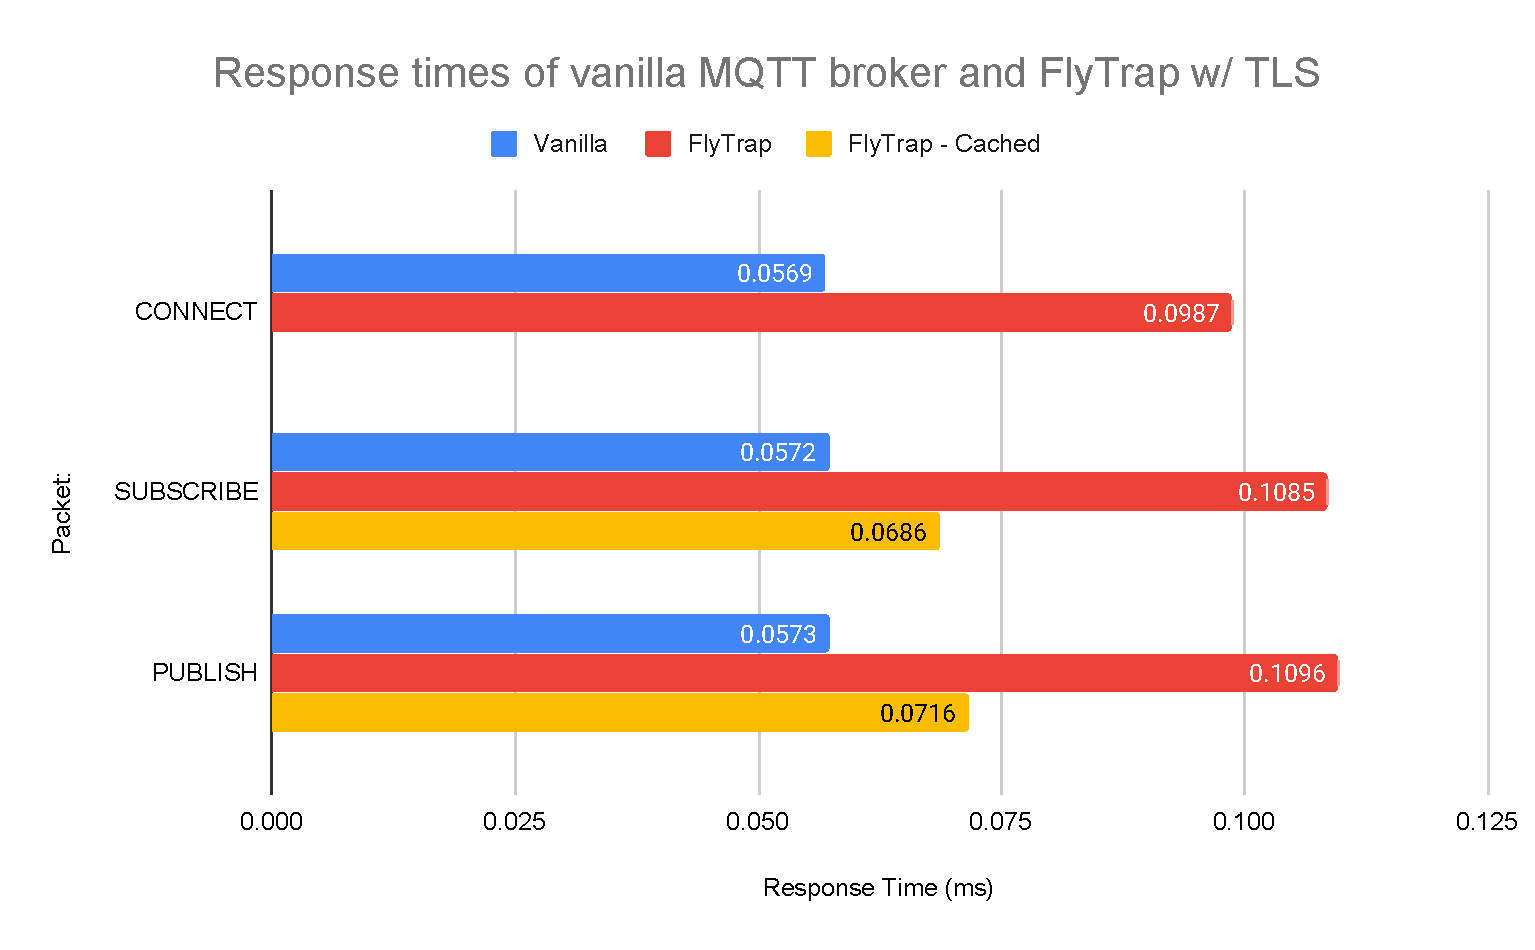
\includegraphics[width=\textwidth]{latency_tls}
    \caption{Response times of most common MQTT requests via a connection with SSL/TLS encryption.}
    \label{fig:latency_tls}
\end{figure}

Statistical tests have been performed on all three datasets. Each of the 100 results for every packet has been compared with the counterpart, for example, 100 CONNECT response times via Vanilla Broker vs 100 CONNECT response times via FlyTrap. This allows us to reject the null hypothesis, as for the first test, the \textit{p-value} is $<0.05$. Tests number 2\ and 3\ resulted with \textit{p-value} $=0$, which can be interpreted as significantly lower than 0.001.

\begin{table}[h]
\centering
\begin{tabular}{|l|l|l|l|}
\hline
\textbf{\#} & \textbf{Test Data}                       & \textbf{Performed Test} & \textbf{p-value}                      \\ \hline
1           & CONNECT: Vanilla vs FlyTrap              & Two Tailed T-Test       & $2.16*10^{-69}$                    \\ \hline
2           & SUBSCRIBE: Vanilla vs FlyTrap vs Cached & Kruskal-Wallis          & $<<< 0.001$ \\ \hline
3           & PUBLISH: Vanilla vs FlyTrap vs Cached & Kruskal-Wallis          & $<<< 0.001$ \\ \hline
\end{tabular}
\caption{Outcome of statistical tests on each of the MQTT packets considered for TLS-encrypted connection.}
\label{tab:ttest-tls}
\end{table}

\subsection{Plain TCP}
The test above was repeated, this time disabling TLS encryption for both ends of the connection. The first thing that we can notice is the overall decrease in response times when compared with the TLS connection. This is a clear indicator that TLS does indeed add an overhead to standard TCP connections. Experiment results were placed on a bar chart similarly as before. Again, standard error bars were omitted, as they were found to be less than $0.1\%$.

Figure \ref{fig:latency_notls} shows the average response time for each of the packets. When sending the request through FlyTrap, we notice an increase in response time of $18.13\%/43.30\%/31.58\%$ respectively for CONNECT/SUBSCRIBE/PUBLISH packets. For FlyTrap - Cached, when compared with the vanilla broker, this increase was less prominent, showing an increase of $23.41\%/15.55\%$ respectively for SUBSCRIBE/PUBLISH packets. 

\begin{figure}[h]
    \centering
    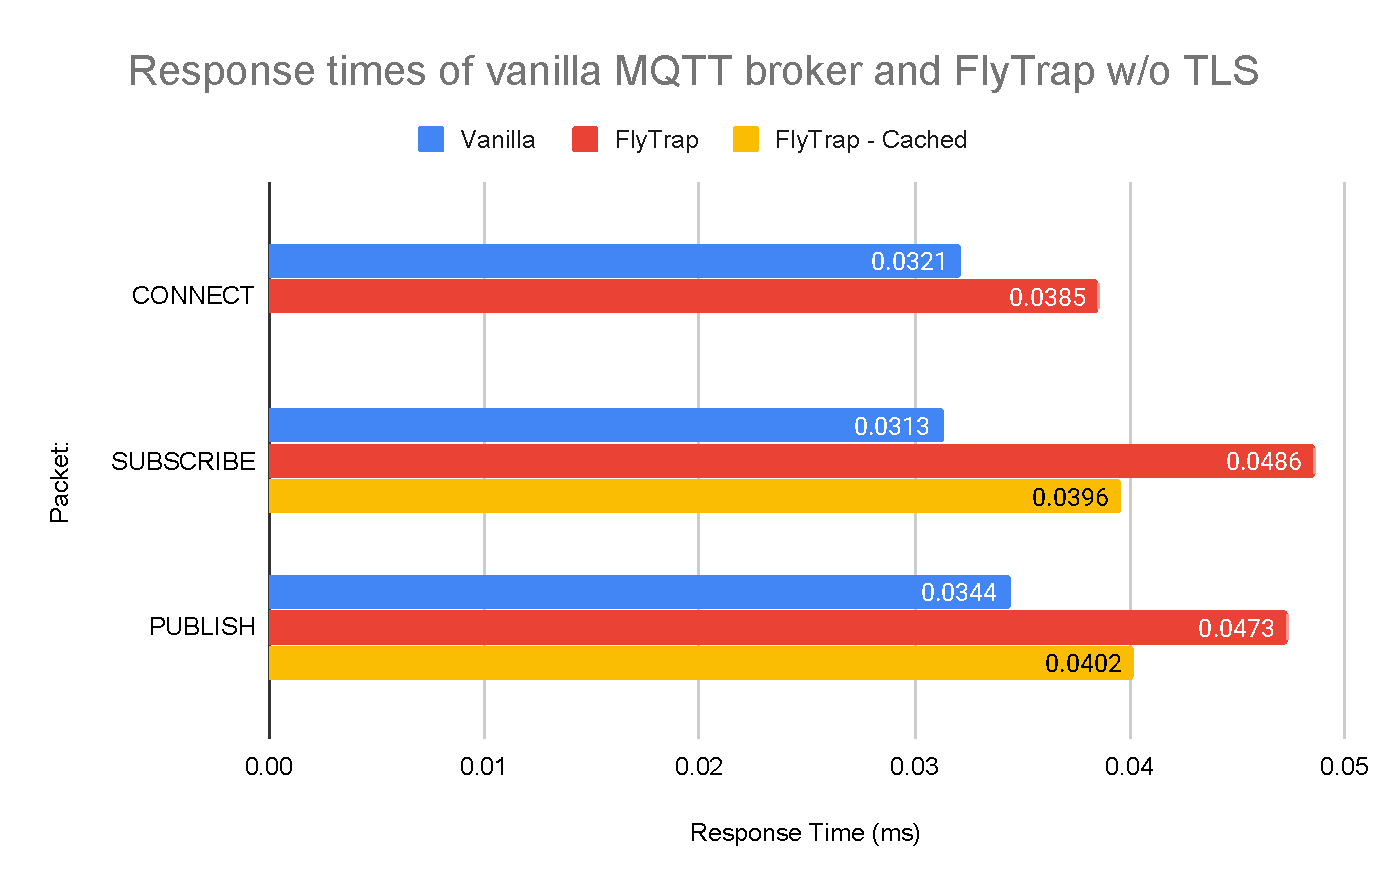
\includegraphics[width=\textwidth]{latency_notls}
    \caption{Response times of most common MQTT requests via a plain TCP connection.}
    \label{fig:latency_notls}
\end{figure}

For each of the tests, the \textit{p-value} was found to be $<0.05$, allowing the null hypotheses to be rejected. Table\ \ref{tab:ttest-notls} shows the values of the performed statistical tests.

\begin{table}[h]
\centering
\begin{tabular}{|l|l|l|l|}
\hline
\textbf{\#} & \textbf{Test Data}                       & \textbf{Performed Test} & \textbf{p-value}                      \\ \hline
1           & CONNECT: Vanilla vs FlyTrap              & Two Tailed T-Test       & $8.60*10^{-20}$                    \\ \hline
2           & SUBSCRIBE: Vanilla vs FlyTrap vs Cached & Kruskal-Wallis          & $<<< 0.001$ \\ \hline
3           & PUBLISH: Vanilla vs FlyTrap vs Cached & Kruskal-Wallis          & $<<< 0.001$ \\ \hline
\end{tabular}
\caption{Outcome of statistical tests on each the MQTT packets considered via a plain TCP connection.}
\label{tab:ttest-notls}
\end{table}


\section{Scalability Evaluation}
In this test, 10/100/1000/10000 concurrent clients were dispatched to PUBLISH a single message, with identical size across all tests, through FlyTrap with TLS enabled. Every client was dispatched at the same time, as a separate process, thus ensuring that they did not interfere with each other. Each identified with a different Public Key, forcing FlyTrap to perform authentication flow. Then the time when PUBACK was received was captured and saved.

\begin{figure}[h]
    \centering
    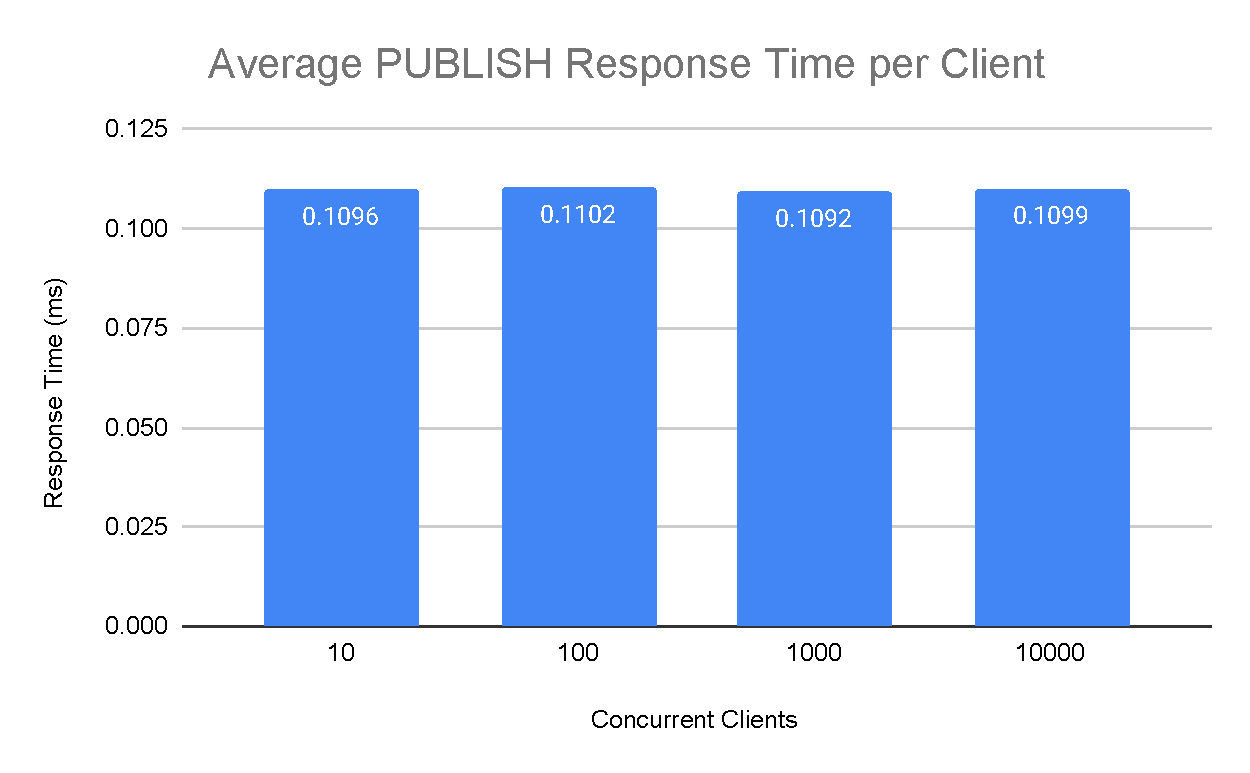
\includegraphics[width=0.8\textwidth]{scale}
    \caption{Average response times with regards to number of concurrent clients.}
    \label{fig:scale}
\end{figure}
See Figure \ref{fig:scale} with the outcome. As with previous tests, standard error has been omitted, as it was less than $0.1\%$. We can see that the response time remains constant across a different number of concurrent clients, with less than $1\%$ change between tests.

\section{Cost Evaluation}
As discussed in Section \ref{sec:poa}, Proof-of-Authority networks do not have any currency involved, and thus there is no reward for mining. However, this removes the benefits of transparency and publicity of the data. On the other hand, running it on a public network (a.k.a. Proof-of-Stake), where miners compete to add new blocks to the network, involves fees and payments and it is essential to keep this cost to the minimum.

\begin{figure}[h]
    \centering
    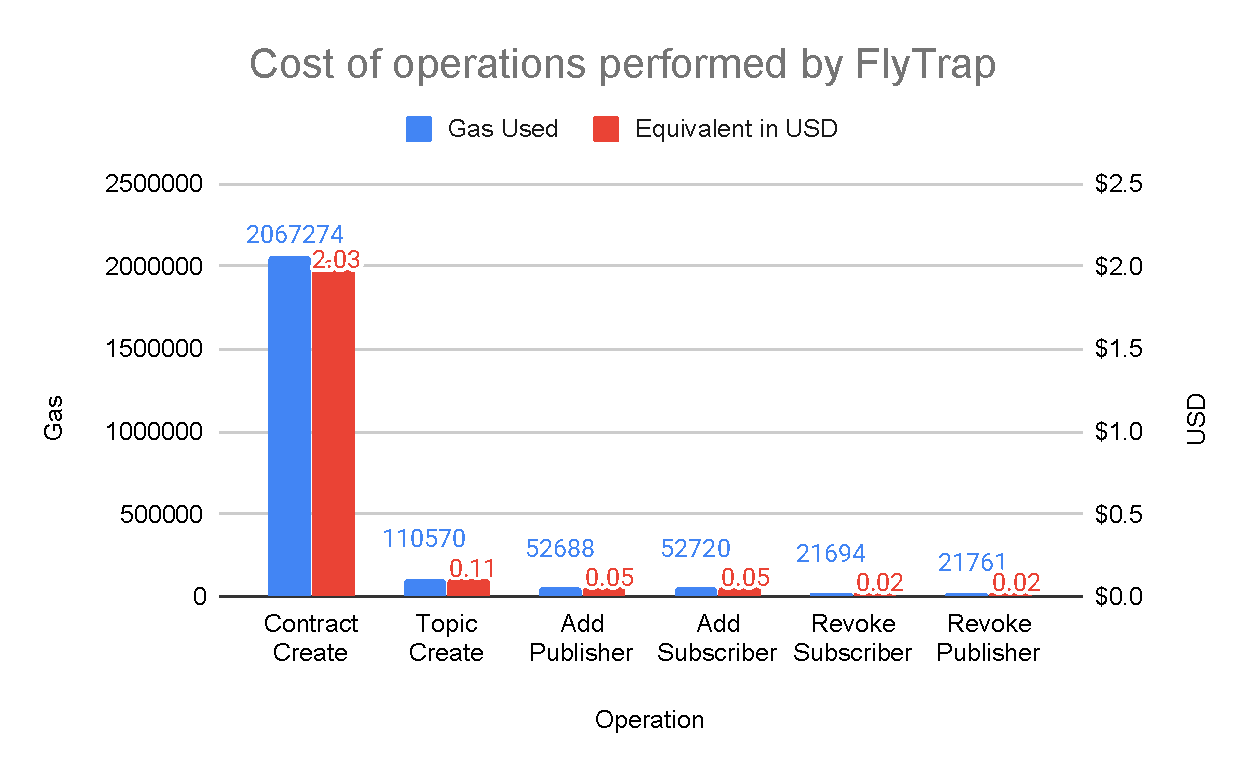
\includegraphics[width=\textwidth]{cost}
    \caption{Cost comparison of various operations on blockchain.}
    \label{fig:cost}
\end{figure}

Six operations performed by FlyTrap were executed a hundred times to extract the average costs in gas. To put those numbers into perspective, the equivalent value in USD was also included - assuming relations of 1 ETH = \$182.29 and 1 Gas = 0.0000000054 ETH\footnote{Data from https://ethgasstation.info/ and https://cex.io/eth-usd as of 2020-04-18}.

Figure~\ref{fig:cost} shows the cost in Gas and in USD for each of the six operations. A maximum charge of \$2.03 and a minimum of \$0.02 is noticed. However, it is important to point out that contract creation occurs only once, when setting up the system. As it allocates memory space on the network for FlyTrap, it is the most expensive operation. All subsequent actions that are modifying its state are priced at below \$0.10.


\section{Scenarios Evaluation}
The last part of the evaluation, examines whether the produced software addresses the problems stated by the Use-case Scenarios in Chapter 3. This focuses mostly on a walk-through of each of the scenarios, demonstrating how the implemented features satisfy the business need defined in the relevant scenario. Scenario \#5 has been omitted, as the security aspect is be apparent throughout the remaining tests.
\subsection{Setup}
Each scenario shares same number of common setup steps, which sets up the initial network and proxy. Those steps will be summarised here - and can be assumed to be executed prior to any of the subsequent scenarios.
\paragraph{Step 1} - Configure the blockchain. For the sake of this experiment, we use Ganache, which starts a test network, with accounts that have 100 ETH pre-filled currency. Once started, a window similar to Figure~\ref{fig:ganache} appears.
\paragraph{Step 2} - Set endpoint for the blockchain node (Ganache default) and create a new contract for FlyTrap.
\begin{lstlisting}[language=bash]
$ export BLOCKCHAIN_ADDRESS="http://localhost:7545"
$ go run cmd/blockchain/main.go -new -contract=""
2020/04/18 20:28:44 Generated new contract, address is:
0xD0BaD0f1fC6D627E1e6fcE6020De9BbA2507498f
\end{lstlisting}
\paragraph{Step 3} - Set contract as environmental variable, add new topic and add publishers/subscribers.
\begin{lstlisting}[language=bash,breaklines=true]
$ export BLOCKCHAIN_CLIENT="0xD0BaD0f1fC6D627E1e6fcE6020De9BbA2507498f"
$ go run cmd/blockchain/main.go -new_topic "creating test topic" -topic "TopicName"
$ go run cmd/blockchain/main.go -topic "TopicName" -client "<client_pubkey>" -pub "adding test publisher"
$ go run cmd/blockchain/main.go -topic "TopicName" -client "<client_pubkey>" -sub "adding test subscriber"
\end{lstlisting}
\paragraph{Step 4} - Start web server. The can now be accessed website under localhost:8081.
\begin{lstlisting}[language=bash,breaklines=true]
$ go run webapp/main.go
\end{lstlisting}
\paragraph{Step 5} - Finally, ready to start the FlyTrap proxy. The command assumes TLS as default, with summary reports generated every hour, connection to test mosquitto broker and starts accepting connections under port 8888.
\begin{lstlisting}[language=bash,breaklines=true]
$ go run cmd/flytrap/main.go -b-freq=1h
2020/04/18 21:04:15 Now accepting connections under :8888
\end{lstlisting}
\subsection{Scenario \#1}
To recap, the first scenario outlined the need for guarding the access to the data from people outside given jurisdiction, for example, only people within the UK should have access to some designated data, so the access can be governed and regulated to ensure compliance with the law.

In this scenario, we are looking to restrict access to a specific topic, only to people connecting from a country which has been permitted. To do so, we need to slightly modify step 2 from the setup process adding an extra `country' flag to the command, as follows:
\begin{lstlisting}[language=bash,breaklines=true]
$ export BLOCKCHAIN_CLIENT="0xD0BaD0f1fC6D627E1e6fcE6020De9BbA2507498f"
$ go run cmd/blockchain/main.go -new_topic "creating test topic" -topic "RestrictedTopic" -country="GB"
\end{lstlisting}
From now on, only people connecting from British IPs are allowed, everyone else is presented with the following message:
\begin{lstlisting}[language=bash,breaklines=true]
$ go run client.go -pub=20 -tls=false -priv="privkey1.asc"
2020/04/18 21:04:17 Using cached signature & public key
2020/04/18 21:04:17 Publishing message: Here Be Dragons #0
panic: error publishing: The PUBLISH is not authorized.
\end{lstlisting}
This shows how FlyTrap satisfies the need specified by the Scenario \#1 and meets requirement FR8. Normally, the access the broker would have been allowed, but in this case, FlyTrap captures request coming from outside the UK and blocks the access.
\subsection{Scenario \#2}
This scenario requires us to determine who accessed the requested resource on the specific day, so we can determine the scope of the leak. Once the steps in the setup have been completed (in particular, the `freq' option) and the leak happens, we are ready to inspect the website.

\begin{figure}[h]
    \centering
    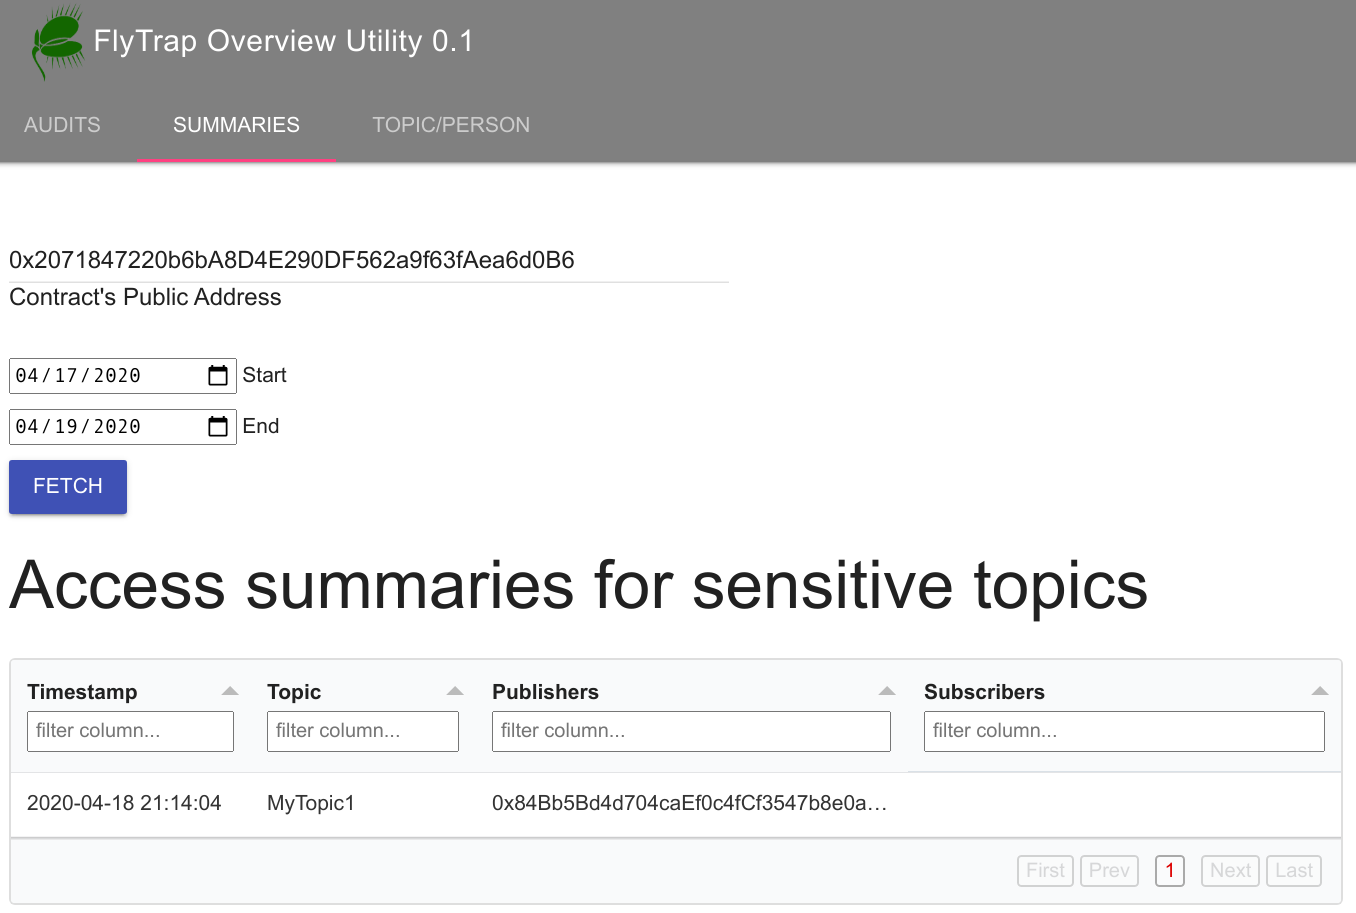
\includegraphics[width=0.9\textwidth]{scenario2}
    \caption{FlyTrap sensitive topics report.}
    \label{fig:scenario2}
\end{figure}

Figure \ref{fig:scenario2} shows how the website would look upon inspecting the access summaries. We can see that on April 18th in the evening, the topic `MyTopic1' was accessed by a single person with the shown public key. Now, we can trace the leakage down to a single person and verify whether their credentials were compromised to assess the damage further.

This then would allow the business affected by the leakage to provide authorities with the list of users that might have been responsible for the unauthorised data access, satisfing requirements stated by General Data Protection Regulation and FR7 specified in Section \ref{sec:func}.

\subsection{Scenario \#3}
Here we are looking to verify who can access a particular resource, the difference from Scenario \#2 is that we are looking at resources that are capable of accessing the data (that not necessariliy made use of those capabilities). This can be then used to track the particular servers\footnote{Which each would have their own public/private key pair allocated.} and ensure that all existing data (now requested to be erased) is actually erased.

Again, after following setup steps, we can go ahead and inspect the ``Topic/Person'' part of the web app, which would allow us to see a list of public keys that can access given the topic, as per Figure \ref{fig:scenario3}. Then, the system administrator would be able to correlate the public key with the piece of infrastructure accessing the information and ensure that the access is revoked followed-up with data cleanup (which is covered by FlyTrap, as it is possible that some other unrelated services might have accessed the information).

In the end, this helps us to ensure compliance with GDPR, to be exact, ``Right to be forgotten''. Normally, those servers might be distributed across the network and since MQTT Brokers do not save access logs, finding them might be challenging. This also proves how FR7 is satisfied.
\begin{figure}[h]
    \centering
    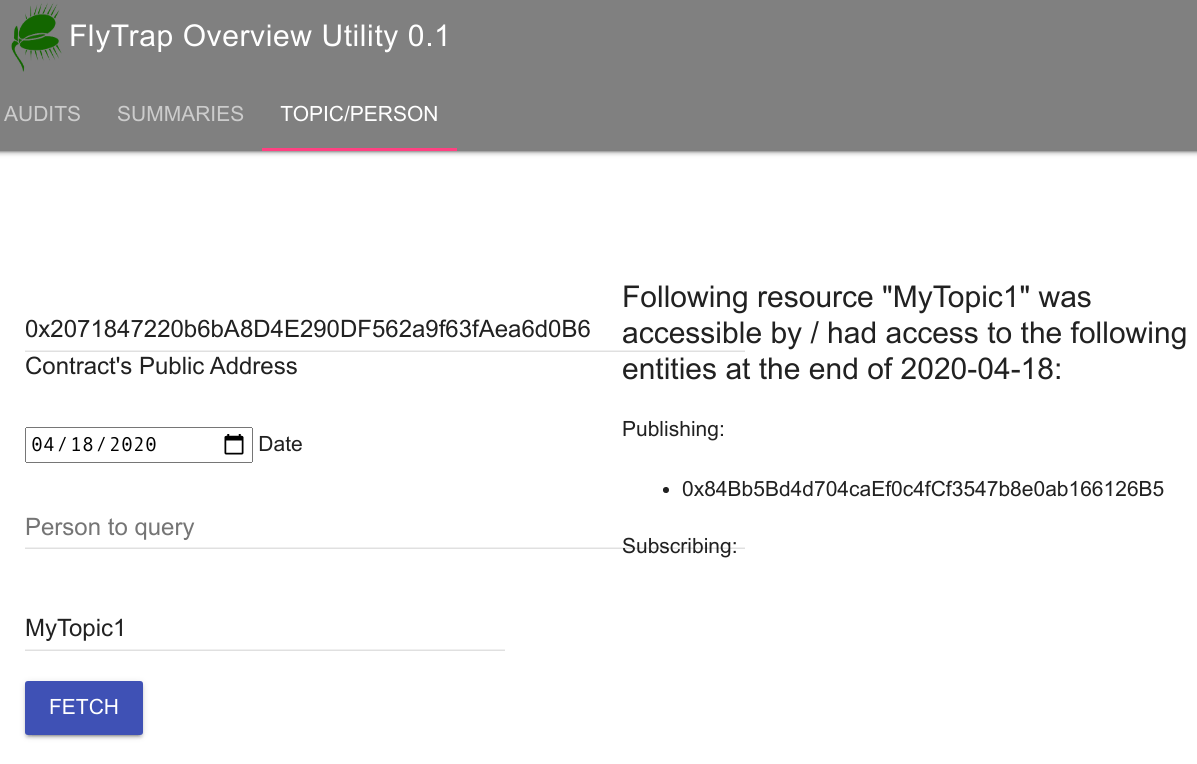
\includegraphics[width=0.9\textwidth]{scenario3}
    \caption{Current Access Control List Summary.}
    \label{fig:scenario3}
\end{figure}
\section{Results}
\subsection{Latency Evaluation}
The overhead added by FlyTrap is apparent, reaching an extra 0.05ms per request. Though, it is interesting to see - looking at the ``FlyTrap - Cached'' bar in Figure \ref{fig:latency_tls} \& \ref{fig:latency_notls} - that caching remediates this problem almost completely, reducing the average response time by up to 37\%, negating the overhead introduced by the first request. We can conclude that FlyTrap would be the most efficient for situations where it is not restarted very often, allowing the cache to grow and in order to minimise the impact for clients often connecting to the broker. As expected, we also note longer response times for FlyTrap with TLS enabled. This is most probably caused by the fact that there needs to be two separate TLS sessions established, encrypting/decrypting the data twice.

For FlyTrap with enabled caching functionality, we notice an average increase of 0.009ms across both plain TCP and TLS when compared with a vanilla broker. This is significantly less than the specified 500ms in \textbf{NFR1} and thus meets this non-functional requirement and concludes the first research question: FlyTrap imposes an avarege of extra 20\% overhead (0.03ms) per rerquest, when compared with the vanilla broker.

It is also interesting to see that the increased latency is much larger in TLS connections when compared to TCP. With TLS, not only do we have to deal with an extra overhead of having to contact blockchain to read authentication data, but also perform TLS encryption/decryption twice - the first time when communicating with the client and the second time when communicating with the broker.
\subsection{Scalability Evaluation}
On the machine used for testing the response times remained constant, indicating that the proxy is capable of handling many concurrent clients without significant impact on performance. If desired, multiple FlyTrap instances can also be deployed across many machines - each pointing to the same broker, further enhancing the response times. This concludes the second research question: FlyTrap scales in a constant time\footnote{Implying $O(1)$, where $n$ is the number of concurrent clients}, up to 10000 concurrent clients, with no impact on response times.

It is important to note that FlyTrap has an overall limit of the maximum allowed concurrent connections of 65535 (equal to $2^{16}$). Two limitations enforce this: first, MQTT Protocol can only accept client IDs of at most $2^{16}$ characters long, so naturally, it is not able to proxy more connections than that, since the broker would refuse them; second, FlyTrap operates on Linux TCP ports, with an allowed port range up to 65535. Where the latter problem could be fixed with WebSockets (discussed in the next chapter), the former would remain a limitation.
\subsection{Cost Evaluation}
For the cost evaluation, the most expensive operation would be the creation of the new contract, coming down to \$2.03. The contract contains the bare-bones definition of structures used by FlyTrap, so high price was to be expected. Though, this only needs to be performed once - the contract can be reused for as many topics as it is necessary. The remaining operations (which would also be performed more often), have much lower prices. A company looking to create 10 topics with 100 publishers would be looking at an investment of $\$2.03 + 10 * \$0.11 + 100 * \$0.05 = \$8.13$. This scales linearly, and cost remains the same, regardless of the current size of the contract and amount of pre-existing topics/publishers/subscribers.

Blockchain offers a solution with 100\% uptime - and at the same time allowing for potential monetisation data access. The average cost is significantly higher, when compared to centralised solutions, such as SQL server hosted in the cloud - but it lacks the benefits of a distributed ledger. Ultimately, all pros and cons would need to be considered before deciding to utilise Ethereum as a data layer. This concludes the third research question: FlyTrap imposes a one-off network fee of \$2.03 with the subsequent operations costing between \$0.02 and \$0.11, which need to be performed ten times a day maximum.
\subsection{Scenario Evaluation}
Each of the scenario walkthroughs demonstrated how the software fulfils the business needs specified in Section \ref{sec:usecase}, answering the fourth research question. The use-case of Scenarios \#4 illustrated a need for stronger authentication and was omitted, since the setup phase and Scenarios \#1, \#2 and \#3 already made use of authenticating connecting clients using public/private keypairs, thus fulfilling the requirement. For Scenario \#5, please refer to the User Manual (Appendix~\ref{cha:manual}) for an explanation on how to set a cost on adding new publishers or subscribers.

Furthermore, by demonstrating that FlyTrap satisfies Scenarios \#1, \#2 and \#3, we can also deduct that following requirements have been directly satisfied: FR1, FR2, FR6, FR7, FR8 and the following requirements have been indirectly satisfied: FR3, FR4, FR5. 
